\documentclass[11pt,a4paper]{ctexart}
\usepackage[margin=2.2cm]{geometry}
\usepackage{amsmath,amssymb,bm,booktabs,graphicx,float,xcolor,hyperref}
\hypersetup{colorlinks=true,linkcolor=blue!55!black}
\setlength{\parskip}{0.35em}
\title{实验十四：参数化四端子分段高频变压器的 DAB 开关模型与回归验证}
\author{高频变压器可辨识性研究工程}
\date{2026年8月21日}
\begin{document}
\maketitle

\begin{abstract}
本实验在实验十三的 $8+8$ 分段四端子高频变压器基础上，新建独立的双有源桥（DAB）开关模型。模型保留完整对称正定电感矩阵、纵向电容、绕组对地电容及非局部原副边电容矩阵，并以两侧浮置直流母线和单移相（SPS）桥替代线性测试端口。实验记录并解释了浮置副边初始化奇异、理想阶跃激励产生电容冲激以及副边点标记接反三类失效。最终模型采用 $1\,\mu\mathrm{s}$ 有限边沿、$1\,\mathrm{G}\Omega$ 共模数值参考和 $100\,\mathrm{ns}$ Simscape 局部 Backward--Euler 步长，成功完成自动编译和两周期开关回归。该结果验证了拓扑、端口方向、点标记和理想桥功率守恒，但不代表真实器件级 DAB、严格周期稳态或实机参数精度。
\end{abstract}

\section{目的和验收边界}
实验十三用于线性宽频扫频及矩阵/Simscape 交叉验证。本实验不覆盖该基准，而是建立另一模型文件，验证
\[
\text{四端子分段 HFT}\to\text{双侧 SPS 桥}\to
\text{开关波形}\to\text{端口功率回归}.
\]
当前桥是功率守恒的开关函数模型，尚不包含 MOSFET、二极管、死区、$C_{\mathrm{oss}}$、开关损耗和控制闭环。因此本阶段的验收指标是：模型可生成、可编译，波形有界，点标记正确，桥瞬时功率残差接近零，并完整保存失败证据。

\section{分段四端子模型}
一次侧和二次侧各有 8 个串联分段，支路电流写为
\[
\bm i=[\bm i_p^{\mathsf T},\bm i_s^{\mathsf T}]^{\mathsf T}\in\mathbb R^{16}.
\]
磁性支路满足
\begin{equation}
\bm v_b=\bm R\bm i+\bm L\frac{\mathrm d\bm i}{\mathrm dt},
\qquad \bm L=\bm L^{\mathsf T}\succ0 .
\label{eq:rl}
\end{equation}
$\bm L$ 是完整 $16\times16$ 对称正定矩阵，而不是只有一个公共磁通模态的秩一互感近似。电容网络包括分段纵向电容、节点对地电容和 $\bm C_{ps}\in\mathbb R^{8\times8}$。节点 KCL 可写为
\begin{equation}
\bm A\bm i+\bm C_n\frac{\mathrm d\bm v_n}{\mathrm dt}=\bm i_{\mathrm{ext}},
\end{equation}
其中 $\bm A$ 为支路-节点关联矩阵，$\bm C_n$ 由全部电容支路装配。任一跨绕组电容的位移电流为
\begin{equation}
i_{ps,ij}=C_{ps,ij}\frac{\mathrm d}{\mathrm dt}(v_{p,i}-v_{s,j}).
\end{equation}

模型显式保留 $p^+,p^-,s^+,s^-$，差模电压为
\[
v_p=v_{p^+}-v_{p^-},\qquad v_s=v_{s^+}-v_{s^-}.
\]
副边完全浮置时，绝对共模电位未定，$t=0$ 的代数雅可比矩阵奇异。因此只在副边直流负端和参考地之间加入 $1\,\mathrm{G}\Omega$。它用于固定数值规范，不是共同功率回路，也不是把 $s^-$ 和 $p^-$ 硬连接。

\section{开关函数、SPS 和点标记}
\subsection{功率守恒桥}
每个桥用 $u(t)\in[-1,1]$ 表示：
\begin{align}
v_{ac}&=u(t)v_{dc},\\
i_{dc}&=-u(t)i_{ac}.
\end{align}
因此
\begin{equation}
p_{dc}+p_{ac}=v_{dc}i_{dc}+v_{ac}i_{ac}=0.
\label{eq:power}
\end{equation}
$i_{ac}$ 正方向定义为流入桥，所以一次桥向变压器送功率时 $P_{p,ac}<0$，二次桥吸收功率时 $P_{s,ac}>0$。

\subsection{SPS 激励}
开关频率为 $f_s=20\,\mathrm{kHz}$，相移为 $\phi=20^\circ$，直流母线为 $400\,\mathrm{V}/100\,\mathrm{V}$。二次波形延迟
\begin{equation}
\Delta t=\frac{\phi}{2\pi f_s}.
\end{equation}
理想阶跃使 $\mathrm dv/\mathrm dt\to\infty$，于是 $i_C=C\,\mathrm dv/\mathrm dt$ 形成理论冲激。最终模型把 $-1\leftrightarrow+1$ 转换限制为 $1\,\mu\mathrm{s}$，明确避免无穷边沿；该边沿只是数值基线，不代表真实 GaN/SiC 转换过程。

\subsection{副边点标记}
实验十三的 $\bm L$ 用负的一次-二次互感编码点标记，主磁通占优时
\[
v_s\simeq-\frac{v_p}{n},\qquad n\simeq4.
\]
若桥同名端直接相连，则 $+400\,\mathrm{V}$ 与折算后的 $+100\,\mathrm{V}$ 在漏感上相加，引起 kA 级非目标环流。最终版本交换副边交流端子，使非移相区间的折算电压近似抵消。

\section{数值配置和复现}
\begin{table}[H]
\centering
\caption{最终开关回归配置}
\begin{tabular}{ll}
\toprule
项目 & 设置\\
\midrule
分段数 & $N_p=N_s=8$\\
直流电压 & $400\,\mathrm{V}/100\,\mathrm{V}$\\
SPS & $20\,\mathrm{kHz}$，$20^\circ$\\
桥边沿 & $1\,\mu\mathrm{s}$\\
局部求解器 & Backward--Euler，$100\,\mathrm{ns}$\\
仿真/统计窗口 & 2 周期/第 2 周期\\
共模数值参考 & $1\,\mathrm{G}\Omega$\\
\bottomrule
\end{tabular}
\end{table}
进入 \texttt{simulink/} 后依次运行 \texttt{run\_exp14\_build\_compile} 和 \texttt{run\_exp14\_sps\_validation}。代码保存配置、生成 SLX、CSV 汇总、MAT 原始波形和 PNG 图。

\section{结果与功率解释}
桥端功率采用“流入桥为正”。分段网络吸收功率因此为
\begin{equation}
P_{\mathrm{loss}}=-(P_{p,ac}+P_{s,ac}).
\end{equation}
最终编译成功，用时 $6.317\,\mathrm{s}$；第二周期结果如下。
\begin{table}[H]
\centering
\caption{最终回归指标}
\begin{tabular}{lr}
\toprule
指标 & 数值\\
\midrule
一次桥交流吸收功率 & $-48.109\,\mathrm{kW}$\\
二次桥交流吸收功率 & $41.116\,\mathrm{kW}$\\
分段网络吸收功率 & $6.993\,\mathrm{kW}$\\
一次/二次峰值电流 & $211.843/879.960\,\mathrm{A}$\\
一次桥功率残差 & $2.91\times10^{-11}\,\mathrm{W}$\\
二次桥功率残差 & $9.54\times10^{-7}\,\mathrm{W}$\\
核心仿真时间 & $7.199\,\mathrm{s}$\\
\bottomrule
\end{tabular}
\end{table}
一次侧负功率和二次侧正功率与约定一致。式~\eqref{eq:power} 的残差接近机器精度，证明桥元件和端口方向自洽。较大电流源于合成模型仅约 $3.6\,\mu\mathrm{H}$ 总漏感、$20^\circ$ 相移和当前电阻参数，不应解释为实机额定点。

\begin{figure}[H]
\centering
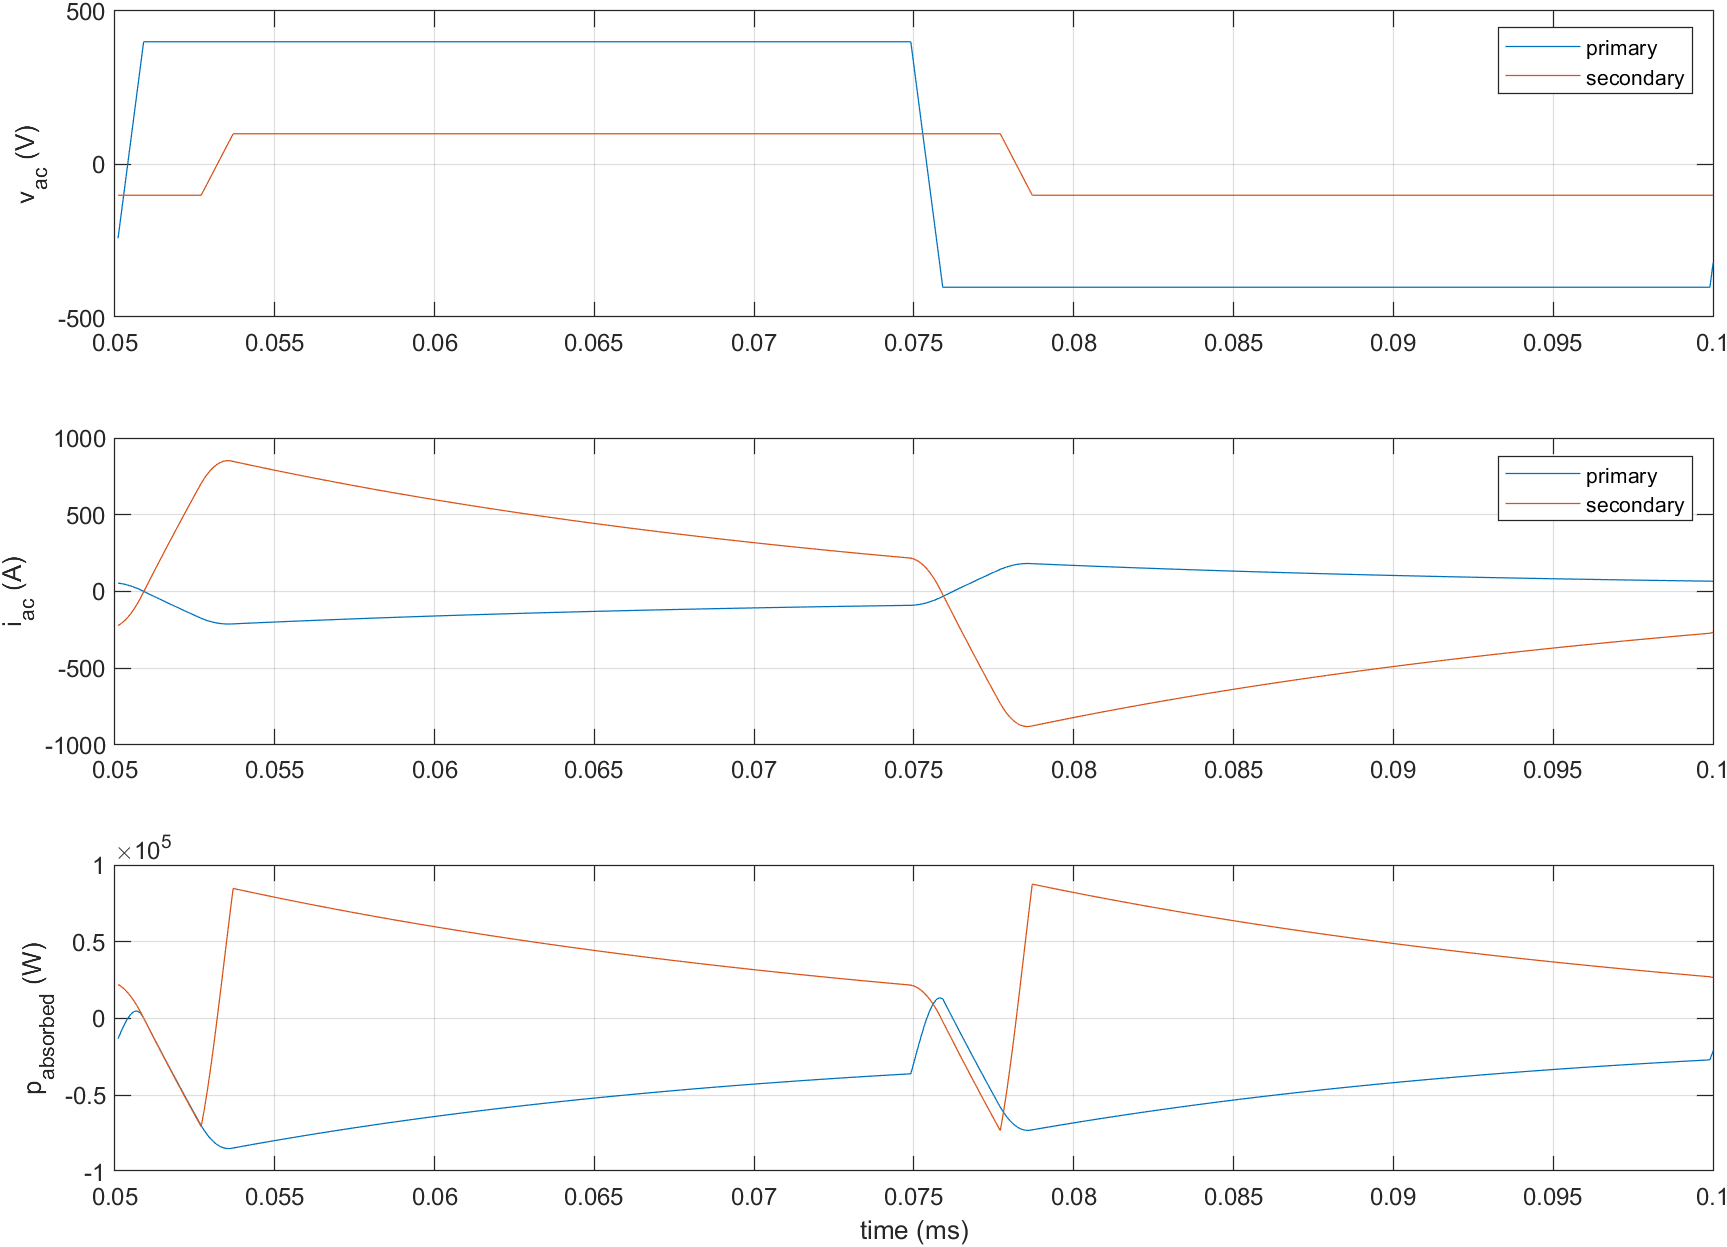
\includegraphics[width=0.97\textwidth]{../figures/sps_switching_regression_waveforms.png}
\caption{第二开关周期的交流端电压、电流和桥吸收功率。}
\end{figure}

\section{失效分析及其价值}
\begin{enumerate}
\item \textbf{浮置初始化奇异：}四端子模型比共同参考二端口多出绝对共模自由度，必须通过真实接地网络或数值规范处理。
\item \textbf{理想阶跃冲激：}原始模型出现 $10^9\,\mathrm{A}$ 量级离散尖峰。失败 CSV、MAT 和图片已用统一的 \texttt{ideal\_edge\_failure} 前缀保留。这说明完整分布电容模型不能与无穷 $\mathrm dv/\mathrm dt$ 的理想桥直接组合。
\item \textbf{点标记接反：}副边未反接时一次/二次峰值约为 $1.1/4.4\,\mathrm{kA}$，说明完整 $\bm L$ 的互感符号必须与外部桥极性统一。
\item \textbf{数值刚性：}全局变步长求解 12 周期超过 7 分钟仍未完成；启用 $100\,\mathrm{ns}$ 局部求解后，两周期核心仿真约 7.2 秒。该现象为后续信息引导分段和模型降阶提供了直接工程动机。
\end{enumerate}

\section{证明了什么，未证明什么}
\subsection*{已经证明}
参数化 $8+8$ 四端子网络能够自动接入双侧浮置 DAB；点标记和端口功率方向已经通过反例及功率残差验证；有限边沿与局部求解器可以得到可重复、有界的短窗波形；现有线性模型和新开关模型已分开保存。

\subsection*{尚未证明}
合成 $\bm R,\bm L,\bm C$ 尚未代表真实样机；两周期不是严格周期稳态，不能报告最终效率或热稳态；桥尚未包含死区、$C_{\mathrm{oss}}$ 和开关损耗；当前尚未显式导出每个内部节点电压及每个 $i_{ps,ij}$；$1\,\mathrm{G}\Omega$ 只是数值参考，不是实际 EMI 接地网络。

\section{下一步}
下一版优先增加内部节点电压和关键跨绕组位移电流测量，然后把实验十二的信息引导降阶模型接入同一 DAB 边界，比较完整 $8+8$ 与降阶模型的端口功率、内部峰值、谐振保持和计算时间。完成后再做多运行窗口
\[
[v_1,i_1,v_2,i_2]_{r=1}^{R}\to\widehat{\bm Y}(\omega)
\to\widehat{\bm\theta},
\]
并用 Fisher 信息决定哪些局部参数可区分、哪些单元必须合并。这样 DAB、分段矩阵和可辨识性分析才能形成统一链路。

\appendix
\section{主要文件}
\begin{itemize}
\item \texttt{simulink/build\_exp14\_dab\_model.m}：模型生成器；
\item \texttt{simulink/make\_exp14\_settings.m}：固定配置；
\item \texttt{simulink/+hftdab/ideal\_switching\_bridge.ssc}：桥元件；
\item \texttt{simulink/generated/hft\_segmented\_dab\_switching\_8p8s.slx}：生成模型；
\item \texttt{results/}：编译、波形、正式结果和失效证据。
\end{itemize}
\end{document}
